\documentclass[a4paper, 12pt]{article}

\usepackage[utf8]{inputenc}
\usepackage[T1]{fontenc}
\usepackage{textcomp}
\usepackage[english]{babel}
\usepackage{amsmath, amssymb}
\usepackage{geometry}
\usepackage{fancyhdr}
\usepackage{hyperref}

\urlstyle{
    colorlinks=true,
    linkcolor=blue,
    filecolor=magenta,      
    urlcolor=cyan,
    %pdftitle={Overleaf Example},
    pdfpagemode=FullScreen,
}


% figure support
\usepackage{import}
\usepackage{xifthen}
\usepackage{pdfpages}
\usepackage{transparent}
\usepackage{graphicx} 
\graphicspath{ {figs/} }
\usepackage{tikz}
\usetikzlibrary{shapes.geometric, arrows}

\tikzstyle{startstop} = [rectangle, rounded corners, minimum width=3cm, minimum height=1cm,text centered, draw=black, fill=red!30]
\tikzstyle{process} = [rectangle, minimum width=3cm, minimum height=1cm, text centered, draw=black, fill=orange!30]
\tikzstyle{decision} = [diamond, minimum width=3cm, minimum height=1cm, text centered, draw=black, fill=green!30]
\tikzstyle{database} = [cylinder, cylinder uses custom fill, 
cylinder body fill=blue!30, cylinder end fill=blue!10,
shape border rotate=90, aspect=0.25, draw]
\tikzstyle{arrow} = [thick,->,>=stealth]


\graphicspath{ {figs/} }
\geometry{left=20mm, top=20mm, bottom=20mm, right=20mm}
\setlength{\parindent}{0pt}
\pagestyle{fancy}
\fancyhead[R]{Rapport SOA}

\usepackage{xcolor}
\usepackage{listings}
\definecolor{codegreen}{rgb}{0,0.6,0}
\definecolor{codegray}{rgb}{0.5,0.5,0.5}
\definecolor{codepurple}{rgb}{0.58,0,0.82}
\definecolor{backcolour}{rgb}{0.97,0.97,0.97}

\lstset{%
  language=bash,
  basicstyle   = \ttfamily\footnotesize,
   backgroundcolor=\color{backcolour}, 
   keywordstyle=\color{magenta},
  keywordstyle = [2]\color{orange},
  commentstyle =    \color{gray}\itshape,
  stringstyle  =   \color{codegreen},
  numbers      = none,
  frame        = single,
   breaklines=true, 
  framesep     = 2pt,
  breakatwhitespace=false, 
   showspaces=false,  
    keepspaces=true, 
  aboveskip    = 1ex
}


\begin{document}
    \thispagestyle{empty}
    \begin{centering}
    \LARGE Voltaired \\
    \Large Rapport de projet SOA\\
    \normalsize
    \vfill
    \textbf{Auteurs:\\}
        Chassignol Valentin\\
        Desmarais Lowen\\
        Giraud Lise\\
        Guilbaud Mathis\\
    \end{centering}
\newpage
\thispagestyle{empty}
    \tableofcontents
\newpage
\pagenumbering{arabic} % reset page numbering

\section{Contexte}

\section{Architecture technique}

\begin{center}
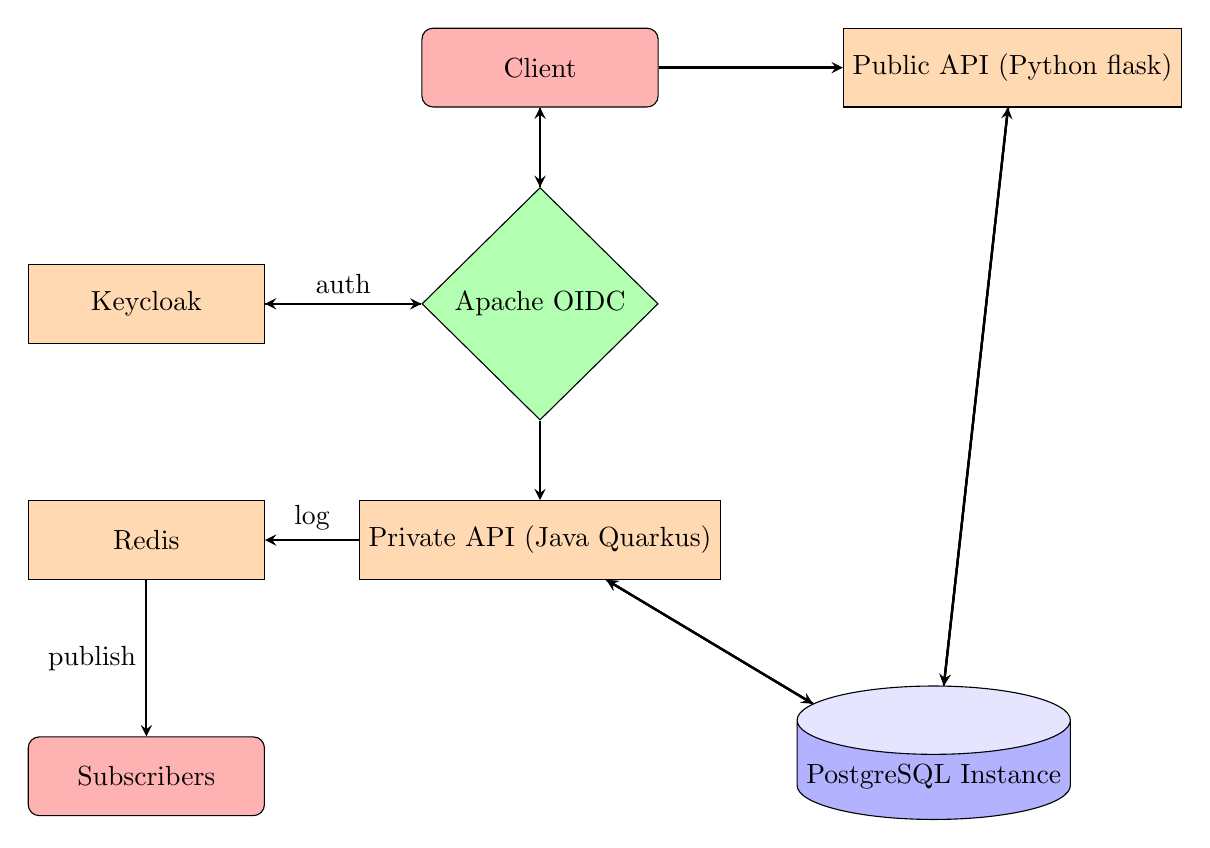
\begin{tikzpicture}[node distance=3cm]
    \node (start) [startstop] {Client};
    \node (rprox) [decision, below of=start] {Apache OIDC};
    \node (api1) [process, right of=start, xshift=3cm] {Public API (Python flask)};
    \node (auth) [process, left of=rprox, xshift=-2cm] {Keycloak};
    \node (api2) [process, below of=rprox] {Private API (Java Quarkus)};
    \node (redis) [process, left of=api2, xshift=-2cm] {Redis};
    \node (sub) [startstop, below of=redis] {Subscribers};
    \node (db1) [database, below of=api2, xshift=5cm] {PostgreSQL Instance};

    \draw [arrow] (start) -- (rprox);
    \draw [arrow] (start) -- (api1);
    \draw [arrow] (api1) -- (db1);
    \draw [arrow] (api1) -- (db1);
    \draw [arrow] (db1) -- (api1);
    \draw [arrow] (db1) -- (api2);
    \draw [arrow] (rprox) -- (start);
    \draw [arrow] (rprox) -- node[anchor=south] {auth} (auth);
    \draw [arrow] (auth) -- (rprox);
    \draw [arrow] (rprox) -- (api2);
    \draw [arrow] (api2) -- (db1);
    \draw [arrow] (db1) -- (api2);
    \draw [arrow] (api2) -- node[anchor=south] {log} (redis);
    \draw [arrow] (redis) -- node[anchor=east] {publish} (sub);
\end{tikzpicture}
\end{center}


\section{Documentation}
\subsection{Installation}

Tout d'abord, afin de pouvoir faire tourner notre application il est 
necessaire d'ajouter un host a votre DNS local, il faut que 
dps.epita.local redirige vers 127.0.0.1

Ensuite nous pouvons debuter l'installation.

\begin{lstlisting}[language=sh]
git clone https://gitlab.cri.epita.fr/lowen.desmarais/voltaired.git
\end{lstlisting}

\subsection{Deploiement}
Pour deployer le projet:
\begin{lstlisting}[language=sh]
cd voltaired
docker compose up -d
\end{lstlisting}

ensuite se connecter sur \url{https://dps.epita.local/}.

Maintenant vous etes assuré que le service tourne, des lors, pour acceder 
aux differentes application il suffit d'utiliser l'un des deux liens suivant:
\begin{itemize}
    \item \url{https://dps.epita.local/java}
    \item \url{https://dps.epita.local/python}
\end{itemize}

\section{Developpement}

\subsection{Structure de la base de donee:}

la base de donnee a ete generee par quarkus a l'aide d'hibernate. Elle
est structuree comme suit:

\begin{figure}[h]
    \centering
    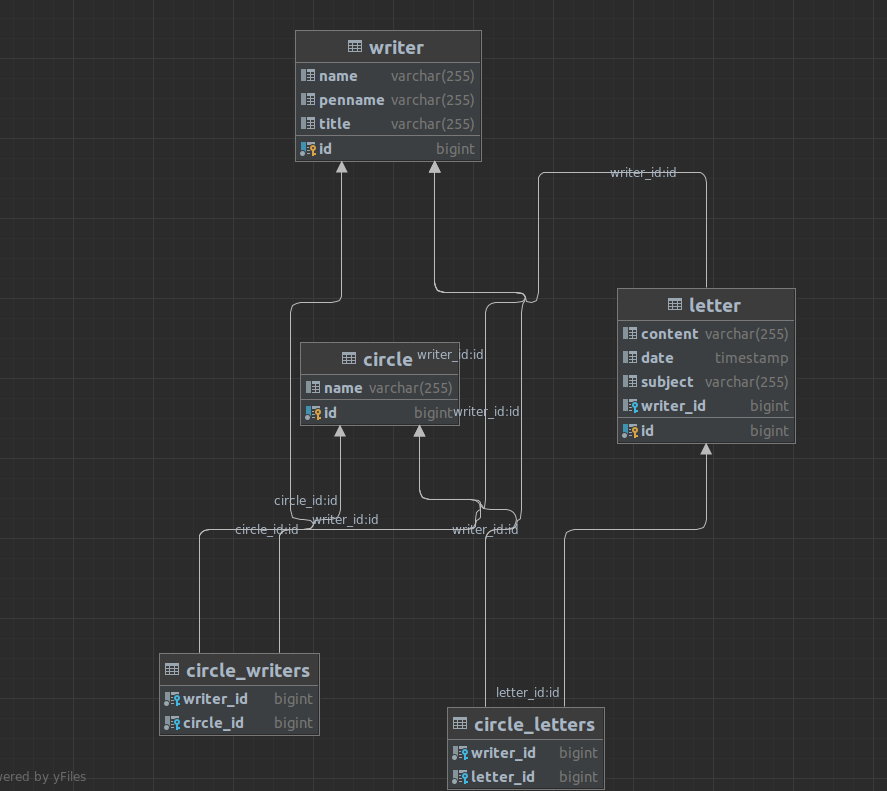
\includegraphics[width=0.6\linewidth]{db}
    \caption{Structure de la DB}
    \label{fig:enter-label}
\end{figure}

\newpage

\subsection{API Publique (Python flask)}

Pour notre projet nous avons tout oriente autour d'un backend fait en 
java avec quarkus. Donc pour creer l'api publique en python il nous a 
fallu nous adapter au format de la db cree par hibernate pour pouvoir 
nous y connecter et faire ainsi toutes les requetes GET.

Pour ce faire, nous avons utilise Flask pour le coeur de l'API, ainsi
que SQLAlchemy en tant qu'ORM. La representation de la DB pour SQLAlchemy est structuree comme suit:
\vspace{1cm}
\begin{lstlisting}[language=python]
from app import db

class Circle(db.Model):
    __tablename__ = 'circle'
    id = db.Column(db.Integer, primary_key=True)
    name = db.Column(db.String(255))

    def __repr__(self):
        return "<Circle {}>".format(self.id)

class Letter(db.Model):
    __tablename__ = 'letter'
    id = db.Column(db.Integer, primary_key=True)
    date = db.Column(db.DateTime)
    subject = db.Column(db.String(255))
    content = db.Column(db.String)
    writer_id = db.Column(db.Integer, db.ForeignKey('writer.id'))
    circle_id = db.Column(db.Integer, db.ForeignKey('circle.id'))
    circle = db.relationship(Circle, backref='letters')

class Writer(db.Model):
    __tablename__ = 'writer'
    id = db.Column(db.Integer, primary_key=True)
    name = db.Column(db.String(255))
    penname = db.Column(db.String(255))
    title = db.Column(db.String(255))
    letters = db.relationship(Letter, backref='writer')
    circles = db.relationship(Circle, secondary='circle_writers')

class CircleWriters(db.Model):
    __tablename__ = 'circle_writers'
    circle_id = db.Column(db.Integer, db.ForeignKey('circle.id'), primary_key=True)
    writer_id = db.Column(db.Integer, db.ForeignKey('writer.id'), primary_key=True)

class CircleLetters(db.Model):
    __tablename__ = 'circle_letters'
    letter_id = db.Column(db.Integer, db.ForeignKey('letter.id'), primary_key=True)
    writer_id = db.Column(db.Integer, db.ForeignKey('writer.id'), primary_key=True) 
\end{lstlisting}



\end{document}
